\section{Introduction}
\label{sec:intro}

Long-context inference has two different scaling problems: the model's active
working set grows with the sequence it rereads, and persistent state grows as more
text is retained.  KV eviction bounds the former by discarding
tokens~\citep{streamingllm,h2o,snapkv} and retrieval bounds it by selecting a
short pack, but both usually retain raw tokens or full-layer KV.  We ask whether
the \emph{depth} axis provides another operating point: can a system retain one
intermediate activation tensor per chunk and reconstruct only the layers above it
when that chunk is retrieved?

CoMem answers this question with a deliberately simple, \emph{training-free}
pipeline on a frozen backbone
(Figure~\ref{fig:architecture}).  A write pass chunks a document, runs each
chunk through layers $[0,j)$ with chunk-local positions, and stores the
$c\times d$ residual activation $h_j$ together with a raw-text BM25 index.  A
read selects fixed top-$k$ chunks, forms
$[\text{sink};h_j^{(1)},\ldots,h_j^{(k)};h_j^q]$ with fresh contiguous
positions, and recomputes layers $[j,L)$ with full cross-pack attention.  This
is neither a fixed-size memory nor an exact transformation of the deployed
input: the persistent hidden/text store is $O(\text{context})$, and relocating
chunk-local $j>0$ states changes the computation.  The narrow benefit is that,
for fixed $k$, model read length is independent of document length; the
measured GPU read-time peak stays approximately flat through 128k (see
Limitations).

\begin{figure*}[t]
    \centering
    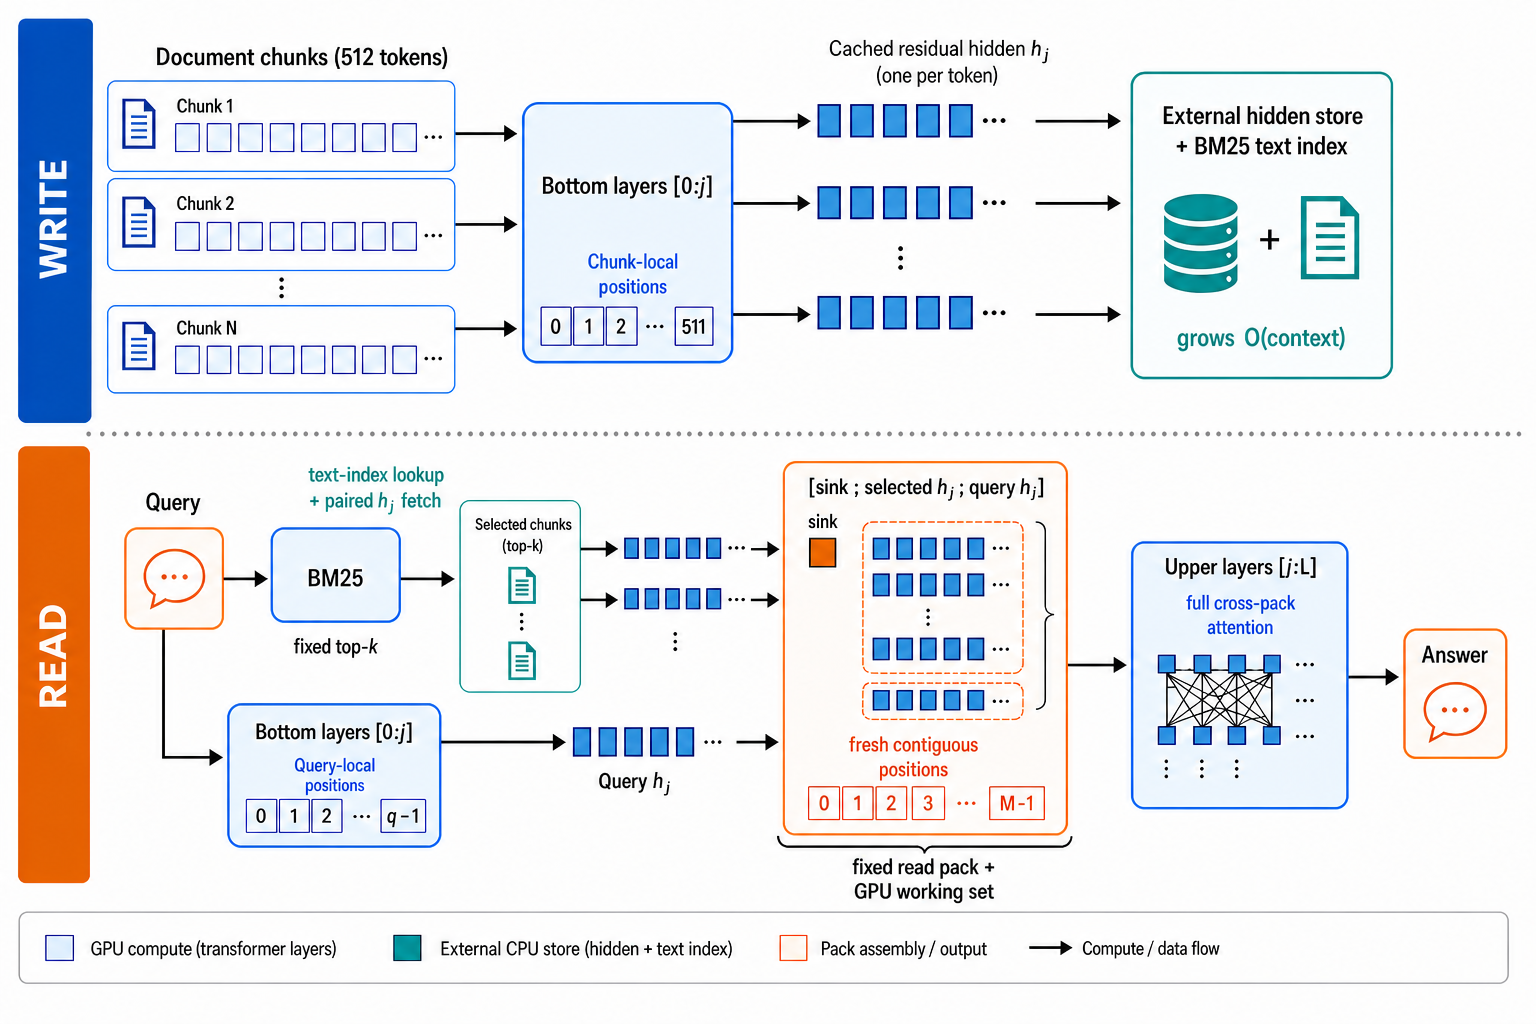
\includegraphics[height=0.19\textheight,keepaspectratio]{figures/comem_architecture_imagegen.png}
    \caption{\textbf{CoMem write--retrieve--read path.}  Each 512-token document
    chunk is written through layers $[0,j)$ and stored as a per-token layer-$j$
    activation with its text-index entry.  BM25 selects fixed top-$k$ chunks; their
    activations and the query activation form a freshly positioned pack read by
    layers $[j,L)$ with full cross-pack attention.  The external store grows as
    $O(\text{context})$; the fixed-$k$ read pack does not (its measured read-time
    peak stays approximately flat through 128k but is not constant).}
    \label{fig:architecture}
\end{figure*}

The central experimental question is consequently not whether retrieval helps,
but what the depth cache contributes \emph{given the same retrieval}.  We
isolate it by comparing $j=12$ with $j=0$ while holding the selected chunks,
query, scorer, and decoder fixed; the $j=0$ arm re-forwards the same retrieved
raw tokens through all layers and is the matched reference.  That comparison
exposes a directional read-out cost rather than a free compression: at the
preregistered BABILong qa1 decision cell the matched $j{=}12$ read is worse than
$j{=}0$ under both the frozen reader and a sensitivity reader that removes
model-generated option enumerations, with the magnitude reported as an interval
rather than a point value (Table~\ref{tab:readdepth-main}).  We therefore treat
depth caching as a quality--systems trade-off, not evidence that a mid-layer
state is a sufficient statistic for general ``understanding.''  A five-arm
decomposition then freezes chunk-independent encoding and position relocation
separately and together: the depth-varying arm remains worse than $j=0$, whereas
relocation is null at the scored endpoint.  This isolates depth with respect to
those named factors, while a residual lower-band context-set difference prevents a
fully deconfounded causal interpretation (Section~\ref{sec:attribution}).

\paragraph{Closest work and the gap we fill.}
The closest prior designs are Layer-Condensed KV~\citep{lckv}, which also caches
a single shallow state on the layer axis but lacks top-$k$ retrieval, and
HCache~\citep{hcache} and KV-Direct~\citep{kvdirect}, which restore or replace
state from intermediate activations without document retrieval
(Section~\ref{sec:related}, Appendix~\ref{app:related}).  What this comparison
set does not provide is a matched, preregistered measurement that holds retrieval,
selector, scorer, and decoder fixed while changing cache depth and reports the
resulting quality cost.  We provide that measurement: an overall downward trend
with a consistent directional loss at the registered comparisons.  CoMem is the
vehicle on which the protocol runs rather than the contribution by itself.  Our
empirical positioning is internal---full
context, matched $j{=}0$, cached $j{=}12$, and the author re-forward controls; a
same-bed comparison to a prior system is not run and remains future work.

\paragraph{Contributions.}
\begin{itemize}
    \item a \textbf{controlled measurement protocol} factorizing depth from
    retrieval, selection, and decoding on a frozen, training-free stack, so the
    depth cache is evaluated as a quality--systems trade-off, not a free
    compression;
    \item a \textbf{depth-cost curve} showing a downward trend under fixed
    retrieval (no tested deeper point recovers $j{=}0$), with matched paired CIs
    and pointwise tests;
    \item a \textbf{measured resource account} separating the $O(\text{context})$
    external store and index from the fixed-$k$ model read, including a 128k H20
    serving comparison and explicit quality losses;
    \item CoMem, the depth-partitioned write--retrieve--read mechanism that
    instantiates the protocol and whose layer-axis store and upper-band
    recomputation are the design we measure.
\end{itemize}
